% !TeX program = xelatex*2
% !TeX root = ../elegantnote.tex
\section{解线性方程组的直接法}
\begin{definition}[特征值和谱半径]
    设$\boldsymbol{A}=(a_{ij})\in \mathrm{R}^{n\times n}$,若存在一个数$\lambda$(实数或复数)和非零向量$\boldsymbol{x}=(x_1,\cdots,x_n)^{\mathrm{T}}\in \mathrm{R}^n$,使
    \[
        \boldsymbol{Ax}=\lambda \boldsymbol{x}
    \]
    则称$\lambda$为$\boldsymbol{A}$的特征值,$\boldsymbol{x}$为$\boldsymbol{A}$对应$\lambda$的特征向量,$\boldsymbol{A}$的全体特征值称为$\boldsymbol{A}$的谱,记作$\sigma(\boldsymbol{A})$,即$\sigma(\boldsymbol{A})=\{\lambda_1,\cdots,\lambda_n\}$,
    \[
        \rho(\boldsymbol{A})=\max_{\lambda\in\sigma(\boldsymbol{A})}|\lambda| 
    \]
    称为$\boldsymbol{A}$的谱半径。
\end{definition}
\begin{definition}
    设$\boldsymbol{u},\boldsymbol{v}\in\mathbb{R}^n,\sigma$为实数,则
    \[
        E(\boldsymbol{u},\boldsymbol{v},\sigma)=\boldsymbol{I}-\sigma\boldsymbol{u}\boldsymbol{v}^{\mathrm{T}}
    \]
    称为初等矩阵。

    \colorbox{cyan!50}{初等矩阵} = \colorbox{red!50}{单位矩阵}减去\colorbox{orange!50}{秩最多为1的方阵}
\end{definition}
\begin{note}
    记$\boldsymbol{u}= ( u_1, u_2, \cdots , u_n)^\mathrm{T}$, $\boldsymbol{v} = ( v_1, v_2, \cdots , v_n)^\mathrm{T}$
    则
    \[
        E(\boldsymbol{u},\boldsymbol{v},\sigma)=(\delta_{ij}-\sigma u_iv_j)_{n\times n}    
    \]

    \begin{enumerate}
        \item 初等矩阵的逆矩阵 
        \[
            E^{-1}(\boldsymbol{u},\boldsymbol{v},\sigma) = I- \beta \boldsymbol{u}\boldsymbol{v}^{T}
        \]
        其中$\beta = \dfrac{\sigma}{\sigma\boldsymbol{v}^{\mathrm{T}}\boldsymbol{u}-1}$
        \item 其行列式
        \[
            \operatorname{det}(E(\boldsymbol{u},\boldsymbol{v},\sigma))=1-\sigma \boldsymbol{v}^{\mathrm{T}}\boldsymbol{u}
        \]
    \end{enumerate}
\end{note}
\begin{definition}[初等-k下三角矩阵(或Gauss变换)]
    设
    \[
        \boldsymbol{l}_k=
        \begin{pmatrix}
            0\\\vdots\\0\\m_{k+1}\\\vdots\\m_n
        \end{pmatrix}
        ,\quad 
        \boldsymbol{e}_k=
        \begin{pmatrix}
            0\\\vdots\\0\\1\\0\\\vdots\\0
        \end{pmatrix} 
    \]
    称矩阵$\boldsymbol{L}_{k}(\boldsymbol{l}_{k}) = E(\boldsymbol{l}_k,\boldsymbol{e}_k,1) = \boldsymbol{I}-\boldsymbol{l}_{k}\boldsymbol{e}_k^{\mathrm{T}}$的初等-k下三角矩阵(或Gauss变换)
    \[
        \begin{aligned}
            \boldsymbol{L}_{k}(\boldsymbol{l}_{k}) &= E(\boldsymbol{l}_k,\boldsymbol{e}_k,1) = \boldsymbol{I}-\boldsymbol{l}_{k}\boldsymbol{e}_k^{\mathrm{T}}\\
            &=\begin{bmatrix}
                1   &     &     &     &     &  \\
                & \ddots &     &     &     &  \\
                &     & 1   &     &     &  \\
                &     & -m_{k+1} & 1   &     &  \\
                &     & \vdots &     & \ddots &  \\
                &     & -m_{n} &     &     & 1 \\
            \end{bmatrix}
        \end{aligned}
    \]
    对其逆矩阵$\beta = \dfrac{1}{\boldsymbol{e}^{\mathrm{T}}\boldsymbol{l}-1} = 1$
\end{definition}
\begin{theorem}
    设有向量 $\boldsymbol{x}=(x_1,x_2,\cdots,x_n)^{\mathrm{T}}$,且$x_k\neq 0$,则存在唯一的初等下三角矩阵(指标为$k$)$\boldsymbol{L}_{k}(\boldsymbol{l}_{k}) = E(\boldsymbol{l}_k,\boldsymbol{e}_k,1) = \boldsymbol{I}-\boldsymbol{l}_{k}\boldsymbol{e}_k^{\mathrm{T}}$,使
    \[
        \boldsymbol{L}_k(\boldsymbol{l}_{k})\boldsymbol{x}=
        \begin{pmatrix}
            x_1\\\vdots\\x_k\\0\\\vdots\\0
        \end{pmatrix}\equiv y
    \]
    其中
    \[
        \boldsymbol{l}_{k} = \left( 0,\cdots,0,m_{k+1},m_{n} \right)^{\mathrm{T}}
    \]
    \[
        m_{i} = \dfrac{x_{i}}{x_{k}},\quad \left( i = k+1,\cdots,n \right)
    \]
\end{theorem}
\begin{definition}[初等反射矩阵]
    设 $\boldsymbol{w}\in\mathbb{R}^n$满足$\|\boldsymbol{w}\|_2^2=\boldsymbol{w}^{\mathrm{T}}\boldsymbol{w}=1,\sigma=2$, 称初等矩阵
    \[
        E(\boldsymbol{w},\boldsymbol{w},2)=\boldsymbol{I}-2\boldsymbol{w}\boldsymbol{w}^{\mathrm{T}}\equiv H(\boldsymbol{w})
    \]
    为初等反射矩阵或 Householder 变换。
\end{definition}
\begin{theorem}
    设$H(\boldsymbol{w}) = \boldsymbol{I}-2\boldsymbol{w}\boldsymbol{w}^{\mathrm{T}}$为初等反设矩阵,则
    \begin{enumerate}
        \item $H(\boldsymbol{w})^{\mathrm{T}} = H(\boldsymbol{w})$(对称)
        \item $H(\boldsymbol{w})^{\mathrm{T}} = H(\boldsymbol{w})^{-1}$(正交)
        \item 设$\boldsymbol{A}$为对称阵,那么
        \[
            \boldsymbol{A}_1 = \boldsymbol{H}^{-1}\boldsymbol{A}\boldsymbol{H} = \boldsymbol{HAH}
        \]也是对称的
    \end{enumerate}
\end{theorem}
\begin{note}
    初等反设矩阵的几何意义
    \[
        H(\boldsymbol{w}) = \boldsymbol{I}-2\boldsymbol{w}\boldsymbol{w}^{\mathrm{T}},\quad \|\boldsymbol{w}\|_2^2=\boldsymbol{w}^{\mathrm{T}}\boldsymbol{w}=1,
    \]
    $\boldsymbol{v}'$为$\boldsymbol{v}$关于平面$S$的镜面反设
    \begin{figure}[htbp]
        \centering
        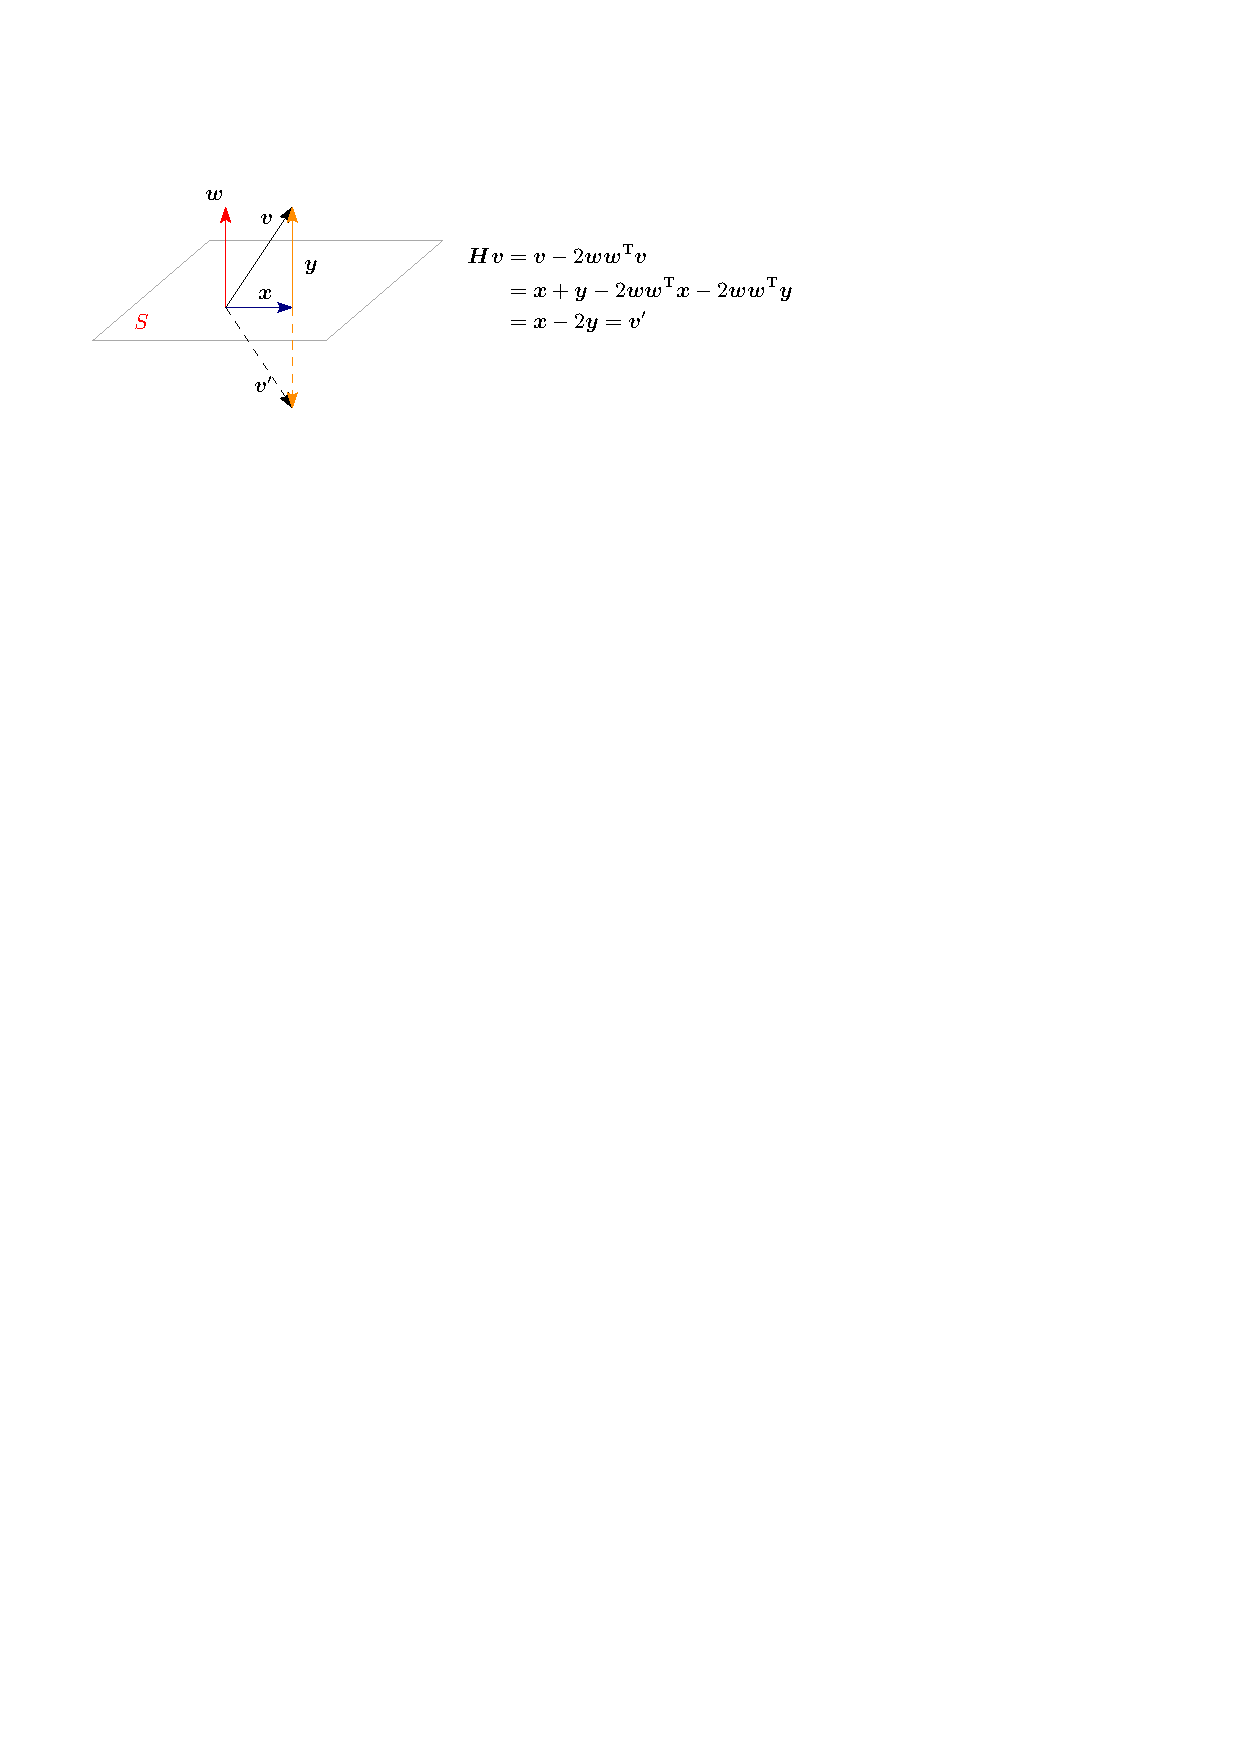
\includegraphics{image/Householder变换.pdf}
    \end{figure}
\end{note}
\subsection{Gauss消元法}
得到等价的线性代数方程组
\[
    \left\{
        \begin{aligned}
            a_{11}^{(1)}x_{1}+a_{12}^{(1)}x_{2}+\cdots+a_{1n}^{(1)}x_{n}=b_{1}^{(1)}\\
            a_{ii}^{(i)}x_{i}+a_{i,i+1}^{(i)}x_{i+1}+\cdots+a_{in}^{(i)}x_{n}=b_{i}^{(i)}\\
            \cdots\\
            a_{n-1,n-1}^{(n-1)}x_{n-1}+a_{n-1,n}^{(n-1)}x_{n}=b_{n-1}^{(n-1)}\\
            a_{nn}^{(n)}x_{n}=b_{n}^{(n)}
        \end{aligned} 
    \right.
\]
    
\begin{algorithm}[h]
    \SetAlgoLined
    \caption{Gauss消元法}
    \label{alg:Gauss}
    \KIN{$[\boldsymbol{A}\,| \boldsymbol{b}]$}
    \KOUT{$\boldsymbol{x}$}
    $\boldsymbol{Z} = [\boldsymbol{A}\,| \boldsymbol{b}]$\\
    \For{$k = 1\to n-1$}{
        \For{$i = k+1\to n$}{
            $\boldsymbol{Z}[i,:]\gets \boldsymbol{Z}[i,:]-\dfrac{a_{ik}^{(k)}}{a_{kk}^{(k)}}\boldsymbol{Z}[k,:]$
        }
    }
    $\boldsymbol{A} = \boldsymbol{Z}[:,1:n]$\\
    $\boldsymbol{b} = \boldsymbol{Z}[:,n+1]$\\
    \For{$i = n\to 1$}{
        $\boldsymbol{x}[{i}] = \boldsymbol{b}[i]$\\
        $\boldsymbol{x}[{i}] = \boldsymbol{x}[{i}]-\boldsymbol{A}[i,i+1:]\boldsymbol{x}[i+1:]$\\
        $\boldsymbol{x}[i] = \boldsymbol{x}[i]/\boldsymbol{A}[i,i]$
    }
    \Return {$\boldsymbol{x}$}
\end{algorithm}
\begin{note}
    高斯消元法的运算量
    \[
        MD = \dfrac{n^3}{3}-\dfrac{n}{3} = \dfrac{n^3}{3} + O(n)
    \]
\end{note}
\begin{example}
    用Gauss消去法解线性方程组(用四位有效数字计算)
    \[
        \left\{\begin{array}{c}0.0001x_1+2x_2=1\\2x_1+3x_2=2\end{array}\right.\boldsymbol{x}^*=\left(\begin{matrix}0.25001875\\0.49998750\end{matrix}\right)
    \]
    \begin{solution}
        用Gauss消去法求解
        \begin{figure}[h]
            \centering
            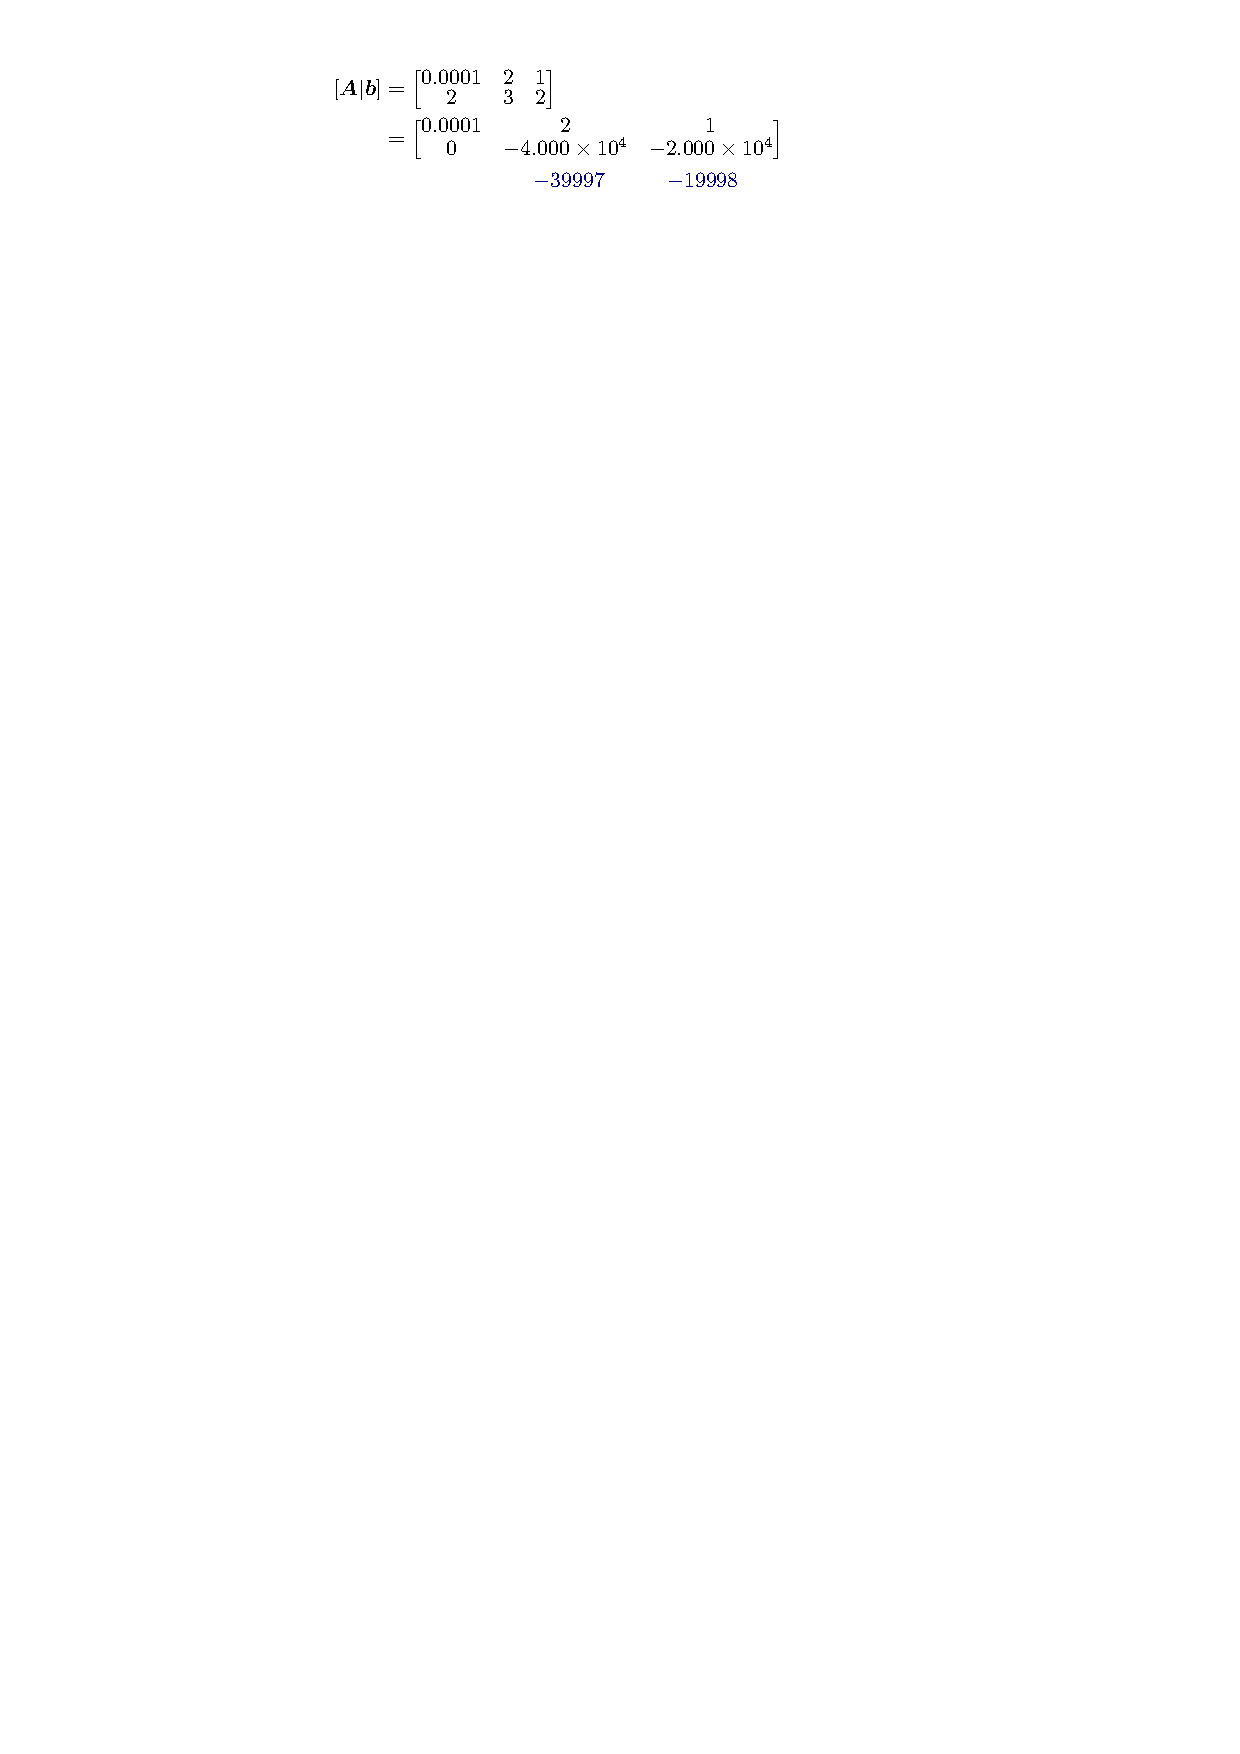
\includegraphics{image/Gauss-example1.pdf}
        \end{figure}
        回代得到$x_1 = 0.0000,\,x_2 = 0.5000$
    \end{solution}
\end{example}
\begin{note}
    问题:

    与精确解相比,该结果相当糟糕
    
    原因:在求行乘数时用了很小的数0.0001作除数
\end{note}
\begin{example}
    将两个方程互换为
    \[
        \left\{
            \begin{array}{rl}
                2x_1+3x_2=2\\
                0.0001x_1+2x_2=1
            \end{array}
        \right.
    \]
    \begin{solution}
        再采用Gauss消去法求解
        \begin{figure}[h]
            \centering
            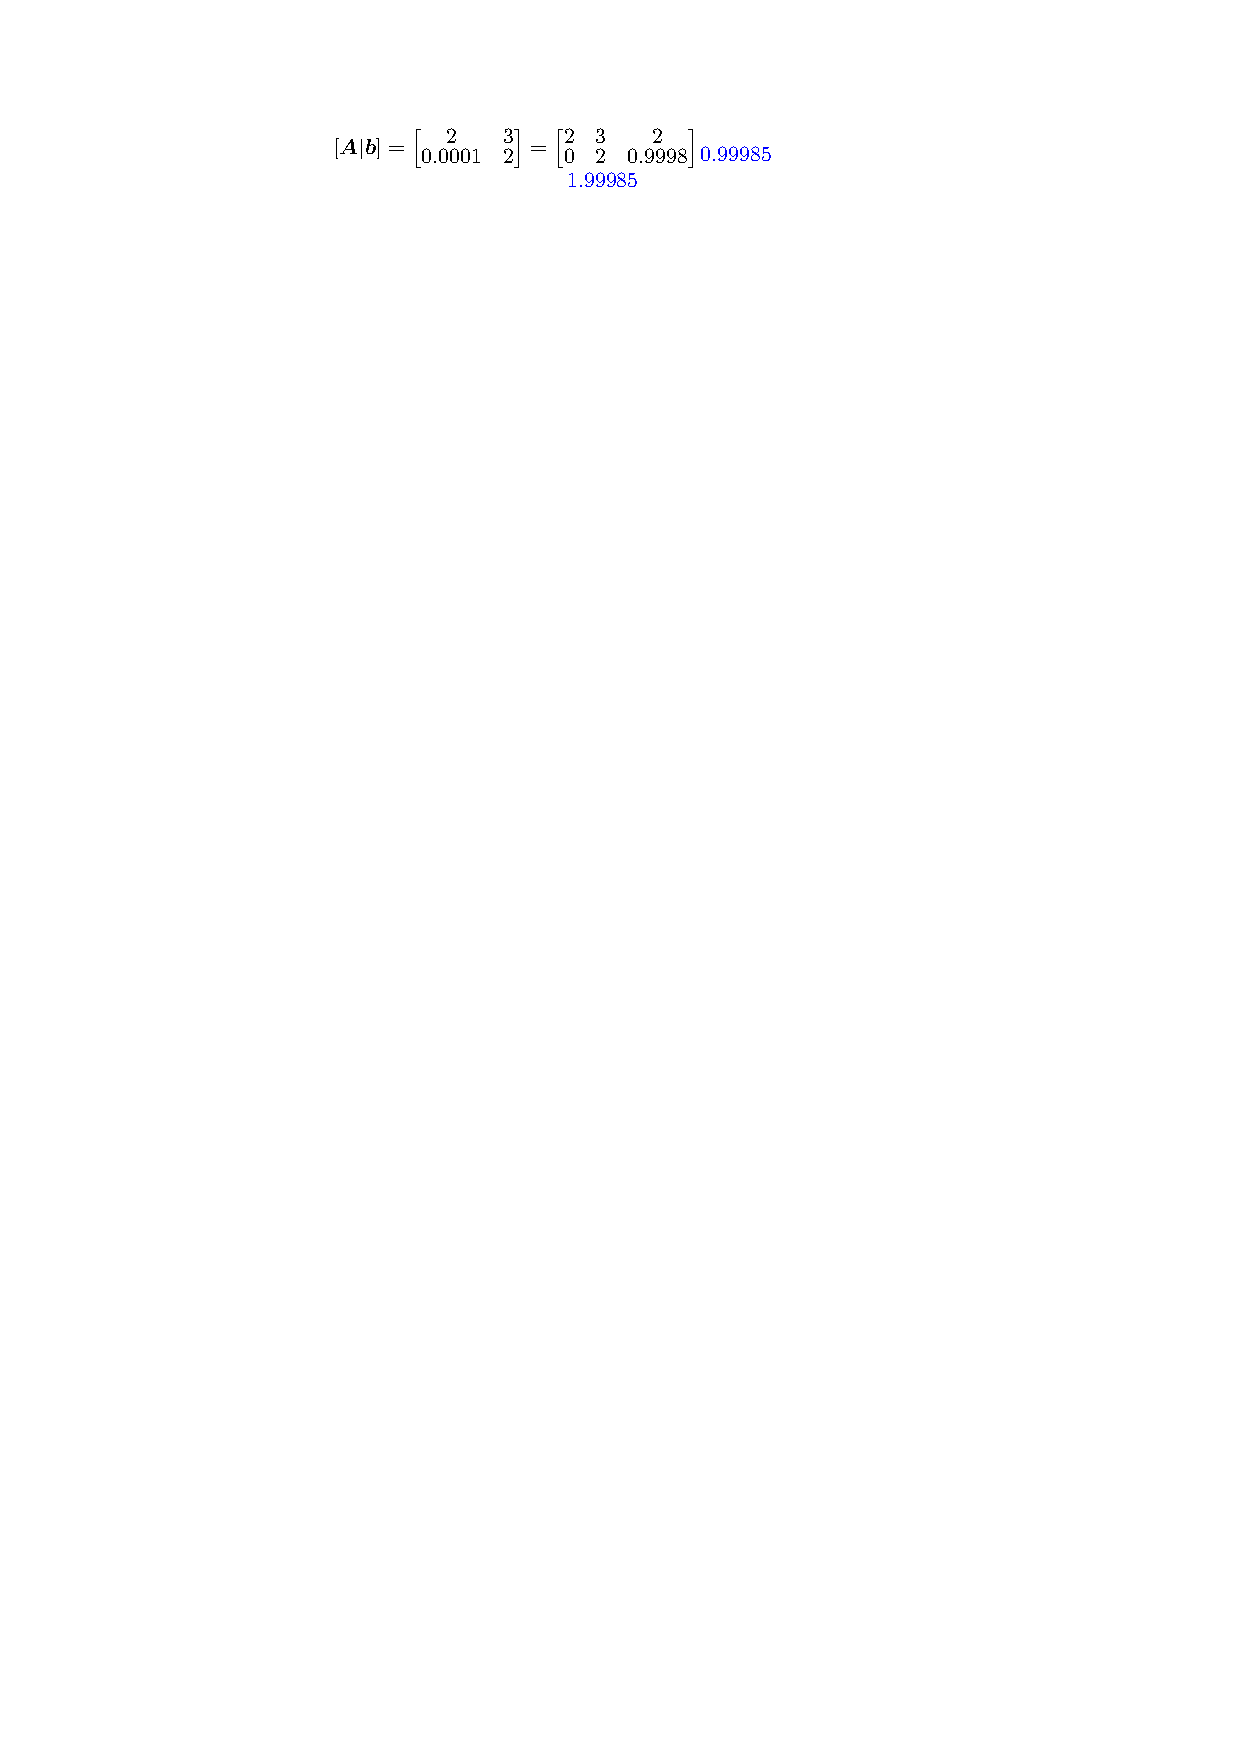
\includegraphics{image/Gauss-example2.pdf}
        \end{figure}
        回代得到$x_1 = 0.2500,\,x_2 = 0.5000$
    \end{solution}
\end{example}
\begin{definition}[列主元Gauss消元法]
    经过$k$步约化后
    \[
        \boldsymbol{A}\to \boldsymbol{A}^{(k)}=
        \begin{bmatrix}
            a_{11}^{(1)} & a_{12}^{(1)} & \cdots & & \cdots & a_{1n}^{(1)}\\
            & a_{22}^{(2)} & \cdots & & \cdots & a_{2n}^{(2)}\\
            & & \ddots & & & \\
            & & & a_{kk}^{(k)} & \cdots & a_{kn}^{(k)}\\
            & & & \vdots & & \\
            \multicolumn{3}{c}{\resizebox{4ex}{!}{$\boldsymbol{0}$}} & a_{mk}^{(k)} & \cdots & a_{mn}^{(k)}
        \end{bmatrix}
    \]
    在$\boldsymbol{A}^{(k)}$的第$k$列选主元,$\mid a_{i_k,k}^{(k)}\mid=\max_{k\leq i\leq n}\mid a_{ik}^{(k)}\mid$。若$i_k>k$,则在$[\boldsymbol{A}^{(k)}\mid \boldsymbol{b}^{(k)}]$中将$i_k$与$k$行互换,再按照Gauss消元公式求出$[A^{(k+1)}\mid b^{(k+1)}]$。重复以上过程直到求出$[\boldsymbol{A}^{(n)}|\boldsymbol{b}^{(n)}]$
\end{definition}
\begin{example}
    要将这段顺序Gauss消元法的Matlab程序改成列主元Gauss消元法,需要在\sol{A} 处添加代码\Stars{3}
    
    \begin{algorithm}[H]
        \SetAlgoLined
        \caption{Gauss列主元消元法}
        \label{alg:GaussElim}
        \KIN{$[\boldsymbol{A}\,| \boldsymbol{b}]$}
        \KOUT{$\boldsymbol{x}$}
        $\boldsymbol{Z} = [\boldsymbol{A}\,| \boldsymbol{b}]$\\
        \For{$k = 1\to n-1$}{
            \tcp*[l]{\colorbox{cyan!50}{A}}
            \For{$i = k+1\to n$}{
                \tcp*[l]{\colorbox{cyan!50}{B}}
                $\boldsymbol{Z}[i,:]\gets \boldsymbol{Z}[i,:]-\dfrac{a_{ik}^{(k)}}{a_{kk}^{(k)}}\boldsymbol{Z}[k,:]$
            }
            \tcp*[l]{\colorbox{cyan!50}{C}}
        }
        $\boldsymbol{A} = \boldsymbol{Z}[:,1:n]$\\
        $\boldsymbol{b} = \boldsymbol{Z}[:,n+1]$\\
        \For{$i = n\to 1$}{
            \tcp*[l]{\colorbox{cyan!50}{D}}
            $\boldsymbol{x}[{i}] = \boldsymbol{b}[i]$\\
            $\boldsymbol{x}[{i}] = \boldsymbol{x}[{i}]-\boldsymbol{A}[i,i+1:]\boldsymbol{x}[i+1:]$\\
            $\boldsymbol{x}[i] = \boldsymbol{x}[i]/\boldsymbol{A}[i,i]$
        }
        \Return {$\boldsymbol{x}$}
    \end{algorithm}
\end{example}
\subsection{直接三角分解法}
经过以下变换
\[
    \boldsymbol{L}_{1}\left(\boldsymbol{l}_{1}\right)= \boldsymbol{I}-\boldsymbol{l}_{1}\boldsymbol{e}_{1}^{\mathrm{T}}
\]
\[
    \boldsymbol{l}_1 = \begin{pmatrix}
        0&\frac{a_{21}}{a_{11}} &\frac{a_{31}}{a_{11}} &\frac{a_{41}}{a_{11}}
    \end{pmatrix}^{\mathrm{T}}
\]
\[
    \boldsymbol{L}_{1}\left(\boldsymbol{l}_{1}\right)=
    \begin{pmatrix}
        1& & &\\
        -\dfrac{a_{21}^{(1)}}{a_{11}^1}& 1 & & \\
        -\dfrac{a_{31}^{(1)}}{a_{11}^1}& & 1 & \\
        -\dfrac{a_{41}^{(1)}}{a_{11}^1}& & & 1 \\
    \end{pmatrix}
    ,\,
    \begin{bmatrix}
        \boldsymbol{A}^{(2)} & \boldsymbol{b}^{(2)}
    \end{bmatrix}  = \boldsymbol{L}_{1}\left(\boldsymbol{l}_{1}\right) 
    \begin{bmatrix}
        \boldsymbol{A}^{(1)} & \boldsymbol{b}^{(1)}
    \end{bmatrix}
\]
\[
    \boldsymbol{L}_{2}\left(\boldsymbol{l}_{2}\right)=
    \begin{pmatrix}
        1 & & &\\
        0 & 1 & & \\
        0 &-\dfrac{a_{32}^{(2)}}{a_{22}^{(2)}}&1&  \\
        0 &-\dfrac{a_{42}^{(2)}}{a_{22}^{(2)}}&&1 \\
    \end{pmatrix}
    ,\,
    \begin{bmatrix}
        \boldsymbol{A}^{(3)} & \boldsymbol{b}^{(3)}
    \end{bmatrix}  = \boldsymbol{L}_{2}\left(\boldsymbol{l}_{2}\right) 
    \begin{bmatrix}
        \boldsymbol{A}^{(2)} & \boldsymbol{b}^{(2)}
    \end{bmatrix}
\]
\[
    \boldsymbol{L'A} = \boldsymbol{U}\Rightarrow\boldsymbol{A} = \boldsymbol{LU}
\]
其中
\[
    \boldsymbol{L}'=\boldsymbol{L}_1(\boldsymbol{l}_2)\boldsymbol{L}_2(\boldsymbol{l}_1)\cdots \boldsymbol{L}_{n-1}(\boldsymbol{l}_{n-1})=\begin{bmatrix}1&&&&\\l_{21}&1&&&\\\vdots&l_{32}&\ddots&&\\\vdots&\vdots&&\ddots&\\l_{n1}&l_{n2}&\cdots&\cdots&1\end{bmatrix}
\]
\begin{theorem}
    设$\boldsymbol{A}\in \mathbb{R}^{n\times n}$非奇异,且各阶顺序主子式
    \[
        D_k=\det\:\boldsymbol{A}_k=
        \begin{vmatrix}
            a_{11}&\cdots&a_{1k}\\
            \vdots&&\vdots\\
            a_{k1}&\cdots&a_{kk}
        \end{vmatrix}\neq0
    \]
    则$\boldsymbol{A}$可唯一地分解为一个单 位下三角阵$\boldsymbol{L}$与一个上三角阵$\boldsymbol{U}$的乘积,即
    \[
        \boldsymbol{A} = \boldsymbol{LU}
    \]
\end{theorem}
\begin{example}
    请将下列矩阵进行三角分解\Stars{3}
    \[
        \boldsymbol{A} = 
        \begin{bmatrix}
            2   & -1  & 3 \\
            4   & 2   & 5 \\
            1   & 2   & 0 \\
        \end{bmatrix}
    \]
    \begin{solution}
        \begin{table}[H]
            \centering
            \begin{tabular}{cc|c|c|c|c|c|c|c|}
                \cline{3-5}\cline{7-9}    第一行 & $\boldsymbol{L}$ & 1   & 0   & 0   & $\boldsymbol{U}$ & \cellcolor[rgb]{ 1,  1,  0}2 & \cellcolor[rgb]{ 1,  1,  0}-1 & \cellcolor[rgb]{ 1,  1,  0}3 \bigstrut\\
                \cline{3-5}\cline{7-9}        &     &     & 1   & 0   &     & 0   &     &  \bigstrut\\
                \cline{3-5}\cline{7-9}        &     &     &     & 1   &     & 0   & 0   &  \bigstrut\\
                \cline{3-5}\cline{7-9}    
        \end{tabular}%
        \end{table}
        \begin{table}[H]
            \centering
            \begin{tabular}{cc|c|c|c|c|c|c|c|}
                \cline{3-5}\cline{7-9}    第一列 & $\boldsymbol{L}$ & 1   & 0   & 0   & $\boldsymbol{U}$ & 2   & -1  & 3 \bigstrut\\
                \cline{3-5}\cline{7-9}        &     & \cellcolor[rgb]{ 1,  1,  0}2 & 1   & 0   &     & 0   &     &  \bigstrut\\
                \cline{3-5}\cline{7-9}        &     & \cellcolor[rgb]{ 1,  1,  0}$\frac{1}{2}$ &     & 1   &     & 0   & 0   &  \bigstrut\\
                \cline{3-5}\cline{7-9}    
            \end{tabular}%
        \end{table}%
        \begin{table}[H]
            \centering
            \begin{tabular}{cc|c|c|c|c|c|c|c|}
                \cline{3-5}\cline{7-9}    第二行 & $\boldsymbol{L}$ & 1   & 0   & 0   & $\boldsymbol{U}$ & 2   & -1  & 3 \bigstrut\\
                \cline{3-5}\cline{7-9}        &     & 2   & 1   & 0   &     & 0   & \cellcolor[rgb]{ 1,  1,  0}4 & \cellcolor[rgb]{ 1,  1,  0}-1 \bigstrut\\
                \cline{3-5}\cline{7-9}        &     & $\frac{1}{2}$ &     & 1   &     & 0   & 0   &  \bigstrut\\
                \cline{3-5}\cline{7-9}    
            \end{tabular}%
        \end{table}%
        \begin{table}[H]
            \centering
            \begin{tabular}{cc|c|c|c|c|c|c|c|}
                \cline{3-5}\cline{7-9}    第二列 & $\boldsymbol{L}$ & 1   & 0   & 0   & $\boldsymbol{U}$ & 2   & -1  & 3 \bigstrut\\
                \cline{3-5}\cline{7-9}        &     & 2   & 1   & 0   &     & 0   & 4   & -1 \bigstrut\\
                \cline{3-5}\cline{7-9}        &     & $\frac{1}{2}$ & \cellcolor[rgb]{ 1,  1,  0}$\frac{5}{8}$ & 1   &     & 0   & 0   &  \bigstrut\\
                \cline{3-5}\cline{7-9}    
            \end{tabular}%
          \end{table}%
          \begin{table}[H]
            \centering
            \begin{tabular}{cc|c|c|c|c|c|c|c|}
                \cline{3-5}\cline{7-9}    第三行 & $\boldsymbol{L}$ & 1   & 0   & 0   & $\boldsymbol{U}$ & 2   & -1  & 3 \bigstrut\\
                \cline{3-5}\cline{7-9}        &     & 2   & 1   & 0   &     & 0   & 4   & -1 \bigstrut\\
                \cline{3-5}\cline{7-9}        &     & $\frac{1}{2}$ & $\frac{5}{8}$ & 1   &     & 0   & 0   & \cellcolor[rgb]{ 1,  1,  0}$-\frac{7}{8}$ \bigstrut\\
                \cline{3-5}\cline{7-9}    
            \end{tabular}%
        \end{table}%
    \end{solution}
\end{example}
\begin{example}
    用Doolittle分解法求解线性方程组\Stars{4}
    \[
        \begin{bmatrix}
            2 & 1 & 1\\
            1 & 3 & 2\\
            1 & 2 & 1\\
        \end{bmatrix}
        \begin{bmatrix}
            x_1\\x_2\\x_3
        \end{bmatrix}
         = \begin{bmatrix}
            4 \\ 6 \\ 5
         \end{bmatrix}
    \]
    \begin{solution}
        \[
            \boldsymbol{L} = \begin{bmatrix}
                1 &&\\
                1/2&1&\\
                1/2&3/5&1
            \end{bmatrix}
            ,\,
            \boldsymbol{U} = \begin{bmatrix}
                2 &1&1\\
                &5/2&3/2\\
                &&3/5
            \end{bmatrix}
        \]
        
        求解$\boldsymbol{Ly} = \boldsymbol{b}$得$\boldsymbol{y} = (4,4,3/5)^{\mathrm{T}}$

        求解$\boldsymbol{Ux} = \boldsymbol{y}$得$\boldsymbol{x} = (1,1,1)^{\mathrm{T}}$
    \end{solution}
\end{example}
\begin{definition}
    若$\boldsymbol{A}\in \mathbb{R}^{n\times n}$对称正定,则存在唯一的对角元为正的下三角矩阵$\boldsymbol{L}$,使$\boldsymbol{A}$分解为
    \[
        \boldsymbol{A} = \boldsymbol{L}\boldsymbol{L}^{\mathrm{T}}
    \]
\end{definition}
\begin{example}
    用平方根法求解线性方程组\Stars{4}
    \[
        \begin{pmatrix}
            4&-1&1\\
            -1&4.25&2.75\\
            1&2.75&3.5
        \end{pmatrix}
        \begin{pmatrix}
            x_1\\x_2\\x_3
        \end{pmatrix}=
        \begin{pmatrix}
            6\\-0.5\\1.25
        \end{pmatrix}
    \]
    则分解后矩阵中的$l_{21}=\sol{-0.5}$。
\end{example}
\subsection{大型带状方程组的求解}
\begin{definition}[三对角方程]
    方程组$\boldsymbol{Ax} = \boldsymbol{f}$称为三对角方程

    其中
    \[
        \boldsymbol{A}=\begin{bmatrix}
            b_1&c_1&&&\\
            a_2&b_2&c_2&&\\
            &a_3&b_3&\ddots&\\
            &&\ddots&\ddots&c_{n-1}\\
            &&&a_n&b_n
        \end{bmatrix},\quad 
        \boldsymbol{f}=\begin{bmatrix}
            f_1\\f_2\\f_3\\\vdots\\f_n
            \end{bmatrix}.
    \]
\end{definition}
\[
    \begin{aligned}
        &\boldsymbol{A}=
        \begin{pmatrix}
            b_1&c_1&&&\\
            a_2&b_2&c_2&&\\
            &\ddots&\ddots&\ddots&\\
            &&a_{n-1}&b_{n-1}&c_{n-1}\\
            &&&a_n&b_n
        \end{pmatrix}\\
        &=\begin{pmatrix}
            \alpha_1&\alpha_1\beta_1&&&\\
            \gamma_2&\gamma_2\beta_1+\alpha_2&\alpha_2\beta_2&&\\
            &\gamma_3&\ddots&\ddots&\\&&\ddots&\gamma_{n-1}\beta_{n-2}+\alpha_{n-1}&\alpha_{n-1}\beta_{n-1}\\
            &&&\gamma_n&\gamma_n\beta_{n-1}+\alpha_n
        \end{pmatrix}
    \end{aligned}
\]
\subsection{向量和矩阵范数}
\begin{definition}
    设$\boldsymbol{x}\in\mathbb{R}^n($或$\boldsymbol{x}\in\mathbb{C}^n)$,关于$\boldsymbol{x}$的某个实值非负函数$N(\boldsymbol{x})\equiv\parallel \boldsymbol{x}\parallel$,如果满足下列条件:
    \begin{enumerate}
        \item $\| \boldsymbol{x}\| \geq 0$,且$\|\boldsymbol{x}\|=0\Leftrightarrow \boldsymbol{x}=0$
        \item $\| \alpha \boldsymbol{x}\| = | \alpha \mid \cdot \| \boldsymbol{x}\| , \alpha \in \mathbb{R} ( \mathbb{C} ) ;$
        \item $\| \boldsymbol{x}+ y\| \leq \| \boldsymbol{x}\| + \| y\| , \forall \boldsymbol{x}, \boldsymbol{y}\in \mathbb{R} ^n( \mathbb{C}^n) .$
    \end{enumerate}
    则称$N(\boldsymbol{x})\equiv\parallel \boldsymbol{x}\parallel$是$\mathbb{R}^n($或$\boldsymbol{x}\in\mathbb{C}^n)$上的一个向量范数(或模)。
\end{definition}
\begin{note}
    常用的向量范数

    有$\boldsymbol{x} = \left( x_1,x_2,\cdots,x_n \right)^{\mathrm{T}}\in\mathbb{R}^n$
    
    \begin{itemize}
        \item $\infty$范数$\|\boldsymbol{x}\|_{\infty} = \max\limits_{1\leq i\leq n}|x_i|$
        \item 1-范数$\|\boldsymbol{x}\|_{1}  = \sum\limits_{i = 1}^{n}|x_i|$
        \item 2-范数$\|\boldsymbol{x}\|_{2}  = \sum\limits_{i = 1}^{n}\left( x_i^2 \right)^{1/2}$
    \end{itemize}
\end{note}
\begin{definition}[向量的$w$范数]
    向量的$w$范数由矩阵$\boldsymbol{w}$诱导
    \begin{enumerate}
        \item 设$N(\boldsymbol{x}) = \|\boldsymbol{x}\|_{v}$是$\mathbb{R}^{n}$上的一个向量范数
        \item 设$\boldsymbol{w}\in\mathbb{R}^{n\times n}$为非奇异矩阵,则$M(\boldsymbol{x})\equiv\|\boldsymbol{x}\|_{w}\equiv \|\boldsymbol{wx}\|_{v}$是$\mathbb{R}^n$上的一个向量范数
    \end{enumerate}
\end{definition}
\begin{definition}[矩阵范数]
    关于矩阵$\boldsymbol{A}\in\mathbb{R}^{n\times n}$的某个实值非负函数$N(\boldsymbol{A})\equiv\parallel \boldsymbol{A}\parallel$,如果满足下列条件:
    \begin{enumerate}
        \item $\parallel \boldsymbol{A}\parallel \geq 0$,且$\parallel \boldsymbol{A}\parallel=0\Leftrightarrow \boldsymbol{A}=0;$
        \item $\parallel \alpha \boldsymbol{A}\parallel = \mid \alpha \mid \cdot \parallel \boldsymbol{A}\parallel , \alpha \in \mathbb{R} ;$
        \item $\parallel \boldsymbol{A}+ \boldsymbol{B}\parallel \leq \parallel \boldsymbol{A}\parallel + \parallel \boldsymbol{B}\parallel , \forall \boldsymbol{A}, \boldsymbol{B}\in \mathbb{R} ^{n\times n};$
        \item $\parallel \boldsymbol{A}\boldsymbol{B}\parallel \leq \parallel \boldsymbol{A}\parallel \cdot \parallel \boldsymbol{B}\parallel , \forall \boldsymbol{A}, \boldsymbol{B}\in \mathbb{R} ^{m\times n}$。
    \end{enumerate}
则称$N(\boldsymbol{A})$是$\mathbb{R}^{n\times n}$上的一个矩阵范数(或模)。
\end{definition}
\begin{definition}[矩阵的F范数]
    $F(\boldsymbol{A})\equiv\|\boldsymbol{A}\|_{F} = \left( \sum\limits_{i,j = 1}^{n}a_{ij}^2 \right)^{1/2}$
\end{definition}
\begin{definition}[矩阵的算子范数]
    设$\boldsymbol{x}\in\mathbb{R}^n,\boldsymbol{A}\in\mathbb{R}^{n\times n}$,已经给出了一种向量范数$\|\boldsymbol{x}\|_{v}$定义一个矩阵的非负函数
    \[
        N(\boldsymbol{A})\equiv\parallel \boldsymbol{A}\parallel_{v}=\max_{\substack{\boldsymbol{x}\in\mathbb{R}^{n}\\\boldsymbol{x}\neq0}}\frac{\parallel \boldsymbol{A}\boldsymbol{x}\parallel_{v}}{\parallel \boldsymbol{x}\parallel_{v}}=\max_{\substack{y\in\mathbb{R}^{n}\\\parallel \boldsymbol{y}\parallel=1}}\parallel \boldsymbol{Ay}\parallel_{v}
    \]
\end{definition}
\begin{note}
    常用的矩阵范数
    
    设$\boldsymbol{x}\in\mathbb{R}^n,\boldsymbol{A}\in\mathbb{R}^{n\times n}$
    \begin{itemize}
        \item $\parallel \boldsymbol{A}\parallel_{\infty}=\max\limits_{1\leq i\leq n}\sum_{j=1}^{n}\mid a_{ij}\mid$,行范数
        \item $\parallel \boldsymbol{A}\parallel_1=\max\limits_{1\leq j\leq n}\sum_{i=1}^n\mid a_{ij}\mid$,列范数
        \item $\parallel \boldsymbol{A}\parallel_2=\sqrt{\rho(\boldsymbol{A}^\mathrm{T}\boldsymbol{A})}$,2-范数
    \end{itemize}
\end{note}
\begin{note}
    矩阵特征值的界
    \begin{enumerate}
        \item 设 $\boldsymbol{A}\in \mathbb{R} ^{n\times n}$,则$\rho(\boldsymbol{A})\leq\parallel \boldsymbol{A}\parallel_v$,
        $\left\|\boldsymbol{A}\right\|_v$为满足相容条件的矩阵范数;
        \item 设$\boldsymbol{A}\in\mathbb{R}^{n\times n}$为对称矩阵,则$\|\boldsymbol{A}\|_2=\rho(\boldsymbol{A})$
    \end{enumerate}
\end{note}
\begin{theorem}
    设$A\in\mathbb{R}^{n\times n},$则
    \[
        \operatorname*{lim}_{k\to\infty}\boldsymbol{A}^{k}=0\Leftrightarrow\rho(\boldsymbol{A})<1
    \]
\end{theorem}
\begin{theorem}
    设$\boldsymbol{B}\in\mathbb{R}^{n\times n}$,且$\parallel \boldsymbol{B}\parallel<1(\parallel \boldsymbol{B}\parallel$为矩阵的算子范数),则 $\boldsymbol{I}\pm \boldsymbol{B}$为非奇异矩阵,且有估计
    \[
        \|(\boldsymbol{I}\pm \boldsymbol{B})^{-1}\|\leq\frac{1}{1-\|\boldsymbol{B}\|}
    \]
\end{theorem}
\begin{proof}
    只证明$\boldsymbol{I}\pm \boldsymbol{B}$为非奇异矩阵,设$\boldsymbol{I}-\boldsymbol{B}$为奇异矩阵,则存在非零向量$\boldsymbol{x}$使得
    \[
        (\boldsymbol{I}+\boldsymbol{B})\boldsymbol{x} = \boldsymbol{0}
    \]
    那么有
    \[
        \begin{aligned}
            \|(\boldsymbol{I}+\boldsymbol{B})\boldsymbol{x}\|&= \|\boldsymbol{x}+\boldsymbol{B}\boldsymbol{x}\|\leq \|\boldsymbol{x}\| + \|\boldsymbol{B}\boldsymbol{x}\|\\
            &\leq \|\boldsymbol{x}\| + \|\boldsymbol{B}\|\|\boldsymbol{x}\| =(1+\|\boldsymbol{B}\|)\|\boldsymbol{x}\|\\
            &<2\|\boldsymbol{x}\|
        \end{aligned}
    \]
\end{proof}
\subsection{条件数与病态矩阵}
\begin{example}
    已知 $A=\begin{pmatrix}1&-3\\-1&2\end{pmatrix}$, 求$\left\|\boldsymbol{A}\right\|_\infty\left\|\boldsymbol{A}\right\|_1,\left\|\boldsymbol{A}\right\|_2.$\Stars{4}
    \begin{solution}
        $\| \boldsymbol{A}\|_{\infty }= 4\| \boldsymbol{A}\|_1= 5$
        \[
            \boldsymbol{A}^\mathrm{T}\boldsymbol{A}=
                \begin{pmatrix}1&-1\\-3&2\end{pmatrix}
                \begin{pmatrix}1&-3\\-1&2\end{pmatrix}
                =\begin{pmatrix}2&-5\\-5&13\end{pmatrix}
        \]
        \[
            \lambda_{1,2}=\frac{15\pm\sqrt{221}}2\quad
            \|\boldsymbol{A}\|_2=\sqrt{\frac{15+\sqrt{221}}2}\approx3.864
        \]
    \end{solution}
\end{example}
\begin{note}
    常用条件数:
    \[
        \mathrm{Cond}(\boldsymbol{A})_{\infty}= \|\boldsymbol{A}^{-1}\|_{\infty}\cdot \| \boldsymbol{A}\|_{\infty}
    \]

    \[
        \begin{aligned}
            &\mathrm{Cond}(\boldsymbol{A})_{2}= \| \boldsymbol{A}^{- 1}\|_{2}\cdot \| \boldsymbol{A}\| _{2} \\
            &= \sqrt{\lambda_{\max}\left(\boldsymbol{A}^{\mathrm{T}}\boldsymbol{A}\right)^{-1}}\cdot\sqrt{\lambda_{\max}\left(\boldsymbol{A}^{\mathrm{T}}\boldsymbol{A}\right)}=\frac{\sqrt{\lambda_{\max}\left(\boldsymbol{A}^{\mathrm{T}}\boldsymbol{A}\right)}}{\sqrt{\lambda_{\min}\left(\boldsymbol{A}^{\mathrm{T}}\boldsymbol{A}\right)}}
        \end{aligned}
    \]
    $\boldsymbol{A}$非奇异、对称,$\|\lambda_1\|\geq\|\lambda_2\|\geq\cdots\geq\|\lambda_n\|$
    \[
        \mathrm{Cond}(\boldsymbol{A})_2=\frac{\|\lambda_1\|}{\|\lambda_n\|}
    \]
\end{note}
\begin{example}
    $\boldsymbol{A}=\begin{bmatrix}1.&1.\\1.&1.0001\end{bmatrix}$的条件数$\operatorname{Cond}(\boldsymbol{A})_{\infty}=$\sol{40000}
    \begin{solution}
        \[
            \boldsymbol{A}=\begin{bmatrix}1.&1.\\1.&1.0001\end{bmatrix}
        \]
        \[
            \boldsymbol{A}^{-1}=\begin{bmatrix}1.0001&-1.\\-1.&1.\end{bmatrix}\cdotp\frac1{0.0001}
        \]
        \[
            \| \boldsymbol{A}\|_\infty=2.0001\quad\| \boldsymbol{A}^{-1}\|_\infty=2.0001\times10^4
        \]
        \[
            \operatorname{Cond}(\boldsymbol{A})_\infty\approx4.\times10^4
        \]
    \end{solution}
\end{example}
\begin{note}
    如何判断$\boldsymbol{Ax} = \boldsymbol{b}$是病态?
    \begin{enumerate}
        \item 估计条件数;
        \item 若用列主元消去法求解方程组$\boldsymbol{Ax} = \boldsymbol{b}$,在约化中出现小主元,可能是病态;
        \item $\boldsymbol{Ax} = \boldsymbol{b}$出现一个相对很大的解,可能是病态;
        \item $\boldsymbol{A}$中的元素的数量级相差很大,可能是病态;
        \item 当$\det(\boldsymbol{A})$相对很小、或$\boldsymbol{A}$某些行(列)近似线性相关,可能是病态
    \end{enumerate}
\end{note}